\documentclass{article}
\usepackage{spconf,amsmath,amssymb,graphicx,booktabs,xcolor}
\usepackage[hidelinks]{hyperref}
\usepackage{enumitem}
\setlist{nosep, leftmargin=12pt}
\setlength{\emergencystretch}{1.5em}

\title{Small regions look homogeneous: finite-sample bias of radiomic texture features and a model-free block-jackknife correction}
\name{Peter Zsoldos}
\address{Tampere University, Tampere, Finland\\ \texttt{peter.zsoldos@tuni.fi}}

\begin{document}
\maketitle

\begin{abstract}
Radiomic texture features such as entropy and GLCM statistics are biased in small regions of interest (ROIs): estimated from few voxels, they make small lesions look homogeneous, so heterogeneity features partly measure lesion size. We present a drop-in wrapper for any feature extractor that removes this bias and flags ROIs where no correction is possible. The bias scales as $c/N$ with a constant set by the image's unknown spatial correlation, which defeats classical corrections; a delete-a-block jackknife over ROI octants cancels it without estimating $c$, and the criterion $N/\xi^3\ge20$, with $\xi$ the correlation length measured in the ROI, decides when the correction is valid. On synthetic textures and 6{,}560 real CT ROIs with an internal reference, including real reconstructions at 1.25--5\,mm, the jackknife removes the joint-entropy bias of 123-voxel ROIs ($-0.63\to-0.01$ bits), cuts its error by up to 59\%, and leaves test--retest repeatability unchanged; across 93 PyRadiomics features it never raises the error of histogram/GLCM features by more than 10\%. We also identify and fix a separate size artefact in PyRadiomics' grey-level discretization.
\end{abstract}

\begin{keywords}
Radiomics, texture analysis, bias correction, jackknife, reproducibility
\end{keywords}

\section{Introduction}
\label{sec:intro}
Radiomics quantifies lesion heterogeneity with texture features computed inside a segmented ROI: first-order entropy and uniformity of the grey-level histogram, and grey-level co-occurrence (GLCM) statistics~\cite{haralick1973}, standardized by IBSI~\cite{zwanenburg2020} and implemented in PyRadiomics~\cite{vangriethuysen2017}. When the ROI is small these \emph{plug-in} estimates are biased---the entropy of an under-sampled histogram is too low---so small lesions look homogeneous for purely statistical reasons. Radiomic features are notoriously confounded with volume~\cite{welch2019}; Brooks and Grigsby~\cite{brooks2014} attributed this to under-sampling and proposed to exclude lesions below a fixed volume, and Shafiq-ul-Hassan et al.~\cite{shafiq2017} proposed empirical normalizations. We found no general correction, and a fixed volume threshold ignores that the information content of an ROI depends on the spatial correlation of the image. Classical entropy corrections, including the jackknife~\cite{miller1955,zahl1977,paninski2003}, assume independent samples, which neighbouring voxels are not.

\noindent\textbf{Contribution.} A drop-in correction for the small-ROI bias of radiomic texture features (Fig.~\ref{fig:overview}). (i) Analysis: the plug-in bias of smooth features is $c/N$ with $c$ inflated by the unknown spatial correlation, so independent-sample corrections under-correct. (ii) Method: a delete-a-block jackknife over ROI octants cancels $c/N$ without estimating $c$ and wraps any extractor unchanged; a per-ROI criterion, $N/\xi^3\ge20$, replaces fixed volume thresholds and flags ROIs where no estimator can work. Block resampling is classical for dependent data~\cite{kunsch1989,lahiri2003}; we found no prior use for this problem, and the criterion is what makes it safe. (iii) Evidence: synthetic textures, 120 real CT regions with an internal reference, real reconstructions, all 93 non-shape PyRadiomics features and 66 lung tumours, including which features cannot be corrected and a second size artefact in PyRadiomics' discretization.



\section{Theory and method}
\label{sec:method}
\noindent\textbf{Plug-in bias under spatial correlation.} Let the image inside an ROI $S$ of $N$ voxels be a stationary random field, and let a texture feature be $\theta=F(\pi)$, a smooth function of a probability vector $\pi$: the grey-level distribution (first order) or the distribution of grey-level pairs at a given offset (GLCM). The plug-in estimate is $\hat\theta_S=F(\hat\pi_S)$, with $\hat\pi_S$ the empirical frequencies in $S$. A second-order expansion gives
\begin{equation}
\mathbb{E}\,\hat\theta_S-\theta\approx\tfrac12\operatorname{tr}\!\big(\nabla^2F(\pi)\,\operatorname{Cov}(\hat\pi_S)\big).
\label{eq:bias}
\end{equation}
For independent voxels $\operatorname{Cov}(\hat\pi_S)=(\operatorname{diag}\pi-\pi\pi^\top)/N$, which for entropy yields the Miller--Madow bias $-(K-1)/(2N\ln2)$ bits for $K$ occupied bins~\cite{miller1955}. For a correlated field, $\operatorname{Cov}(\hat\pi_S)\approx\Sigma_\infty/N$, where the long-run covariance $\Sigma_\infty=\sum_{h}\operatorname{Cov}(e_{X_0},e_{X_h})$ sums the auto-covariances of the bin indicators over all lags $h$. The bias is therefore still $c/N$, but $c$ is inflated by a ``design effect'' roughly equal to the correlation volume $\xi^3$, where $\xi$ is the correlation length. It is unknown and image-dependent, so Miller--Madow-type corrections under-correct.

\begin{figure}[t]
\centering
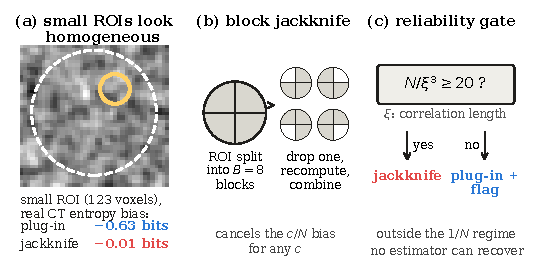
\includegraphics[width=\columnwidth]{figures/fig_overview.pdf}
\caption{Overview. (a) Plug-in entropy of a small ROI is biased low; the jackknife removes the bias. (b) The feature is recomputed without each of $B=8$ contiguous blocks (Eq.~\eqref{eq:jk}). (c) The correction is applied only when the ROI spans enough correlation lengths.}
\label{fig:overview}
\end{figure}

\noindent\textbf{Block jackknife.} Split $S$ into $B$ contiguous blocks $S_b$ (we use $B=8$ octants at equal voxel quantiles along each axis) and recompute the feature on $S\setminus S_b$. If $\mathbb{E}\hat\theta_{S'}=\theta+c/|S'|+o(1/|S'|)$ for every contiguous region $S'$ much larger than $\xi$, the delete-a-group jackknife for unequal groups~\cite{busing1999},
\begin{equation}
\hat\theta_{\text{JK}}=B\,\hat\theta_S-\textstyle\sum_{b}\big(1-\tfrac{n_b}{N}\big)\hat\theta_{S\setminus S_b},\qquad n_b=|S_b|,
\label{eq:jk}
\end{equation}
cancels the $c/N$ term for any $c$, because deleting a contiguous block reduces the effective sample size in proportion to its voxel count. Eq.~\eqref{eq:jk} needs only $B+1=9$ calls of an unmodified extractor and no parameter.

\noindent\textbf{Reliability criterion.} The expansion requires $\operatorname{Cov}(\hat\pi_S)\propto1/N$, i.e.\ an ROI spanning several correlation lengths. When it does not, the ROI samples only part of the texture's variability, the bias is $O(1)$ rather than $O(1/N)$, and no estimator based on the ROI alone can recover $\theta$. We estimate $\xi$ inside the ROI as the lag at which the intensity autocorrelation falls to $1/e$ (averaged over the three axes) and use the effective sample size $N/\xi^3$ as a per-ROI reliability index. Our \emph{gated} estimator returns $\hat\theta_{\text{JK}}$ if $N/\xi^3\ge20$ (threshold from the synthetic study, Sec.~\ref{sec:results}) and otherwise the plug-in value together with an ``unreliable'' flag, since outside the $1/N$ regime the jackknife can add variance without removing bias; this agrees with the theory that a fixed number of subsamples cannot correct severely under-sampled entropies~\cite{jiao2020}.

\noindent\textbf{Bin anchoring.} With a fixed bin width $w$, PyRadiomics assigns grey level $\lfloor x/w\rfloor-\lfloor x_{\min}/w\rfloor+1$, i.e.\ it numbers bins from the ROI minimum $x_{\min}$. Features that use grey-level \emph{values} (GLCM joint/sum average, autocorrelation) then inherit the size dependence of an extreme-value statistic, which shrinks only logarithmically with $N$ and cannot be removed by Eq.~\eqref{eq:jk}. Using absolute bin indices $\lfloor x/w\rfloor$, i.e.\ a fixed anchor, removes it.

\noindent\textbf{Scope.} Eq.~\eqref{eq:bias} covers smooth functionals of histograms and co-occurrences (first order, GLCM), not percentiles (where the jackknife fails), extensive features (energy) or run/zone features (GLRLM, GLSZM, GLDM, NGTDM), whose size dependence is partly definitional.

\section{Experiments}
\label{sec:exp}
\noindent\textbf{Synthetic textures.} Gaussian random fields on $128^3$ grids (Gaussian kernels $\sigma=0.75,1.5,3$ voxels, i.e.\ $\xi=2\sigma$), scaled to CT-like intensities (s.d.\ 60, bin width 25), 10 realizations each. Spherical ROIs of radius 3--14 voxels (123--11{,}513 voxels) are compared with the population value, taken from a radius-60 sphere. We use a NumPy re-implementation of the PyRadiomics first-order and GLCM features, verified to match PyRadiomics~3.0.1 to five decimals.

\noindent\textbf{Real CT regions with an internal reference.} In the 63 CTs of the Medical Segmentation Decathlon lung task~\cite{antonelli2022} we place up to three spheres of radius 14 voxels (about 11{,}500 voxels) entirely inside soft tissue (HU in $[-50,150]$), giving 120 regions from 46 scans. Each large sphere is the reference; ROIs of radius 3--8 voxels are sampled inside it (1{,}045 ROIs). (CT texture and noise, median $\xi$ 0.86 voxels.) To cover smoother textures we repeat the experiment after Gaussian smoothing of the scans ($\sigma=0.7,1.4,2$ voxels; median $\xi=1.6, 3.6, 6.4$; 524, 499, 319 ROIs) and, with real reconstructions, on RIDER Lung CT~\cite{zhao2024rider}, where 32 patients were scanned twice on the same day and each scan was reconstructed with a sharp and a smooth kernel at 1.25, 2.5 and 5\,mm (251 series with uniform slice spacing, 640 regions, 4{,}173 ROIs).

\noindent\textbf{All PyRadiomics features.} On 96 ROIs (radius 4 and 6, from 29 scans) we wrap the unmodified PyRadiomics extractor (93 first-order, GLCM, GLRLM, GLSZM, GLDM, NGTDM features) in Eq.~\eqref{eq:jk}; bias and root-mean-square error (RMSE) are in units of the reference's between-region s.d.

\noindent\textbf{Lung tumours.} For the 66 MSD tumour components (68--338{,}472 voxels, median 6{,}866) we compute all features with and without correction and their Spearman correlation $\rho$ with tumour volume; for the RIDER tumours (radiologist segmentations) we compute test--retest ICC(3,1) per reconstruction.

\begin{figure*}[t]
\centering
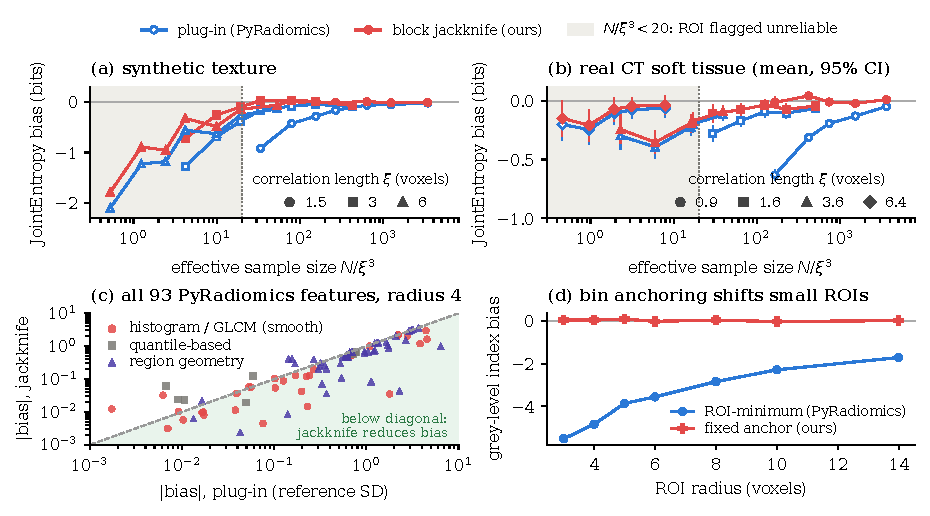
\includegraphics[width=\textwidth]{figures/fig_main.pdf}
\caption{(a,b) Bias of GLCM joint entropy vs.\ effective sample size $N/\xi^3$ on synthetic textures (a) and real CT soft tissue with an internal reference (b); marker shape: correlation regime. (c) Absolute bias of the 93 PyRadiomics features at radius 4, plug-in vs.\ jackknife. (d) Bias of the mean grey-level index under ROI-minimum and fixed bin anchoring.}
\label{fig:main}
\end{figure*}

\begin{table}[t]
\centering\footnotesize
\caption{RIDER real reconstructions (kernel, slice thickness; median $\xi$ in voxels), soft tissue with an internal reference: JointEntropy bias and RMSE (bits) over radii 3--8 voxels for plug-in (PI), block jackknife (JK) and gated jackknife (G; applied to the given share of ROIs).}
\label{tab:real}
\setlength{\tabcolsep}{2.3pt}
\begin{tabular}{@{}lcc ccc ccc@{}}
\toprule
& & & \multicolumn{3}{c}{bias} & \multicolumn{3}{c}{RMSE}\\
\cmidrule(lr){4-6}\cmidrule(l){7-9}
setting & $\xi$ & applied & PI & JK & G & PI & JK & G\\
\midrule
sharp, 1.25\,mm & 0.8 & 100\% & $-0.34$ & $+0.03$ & $+0.03$ & 0.46 & 0.19 & 0.19\\
sharp, 2.5\,mm & 0.8 & 100\% & $-0.33$ & $-0.01$ & $-0.01$ & 0.45 & 0.23 & 0.23\\
sharp, 5\,mm & 0.8 & 100\% & $-0.35$ & $-0.09$ & $-0.09$ & 0.51 & 0.37 & 0.37\\
smooth, 1.25\,mm & 1.1 & 98\% & $-0.17$ & $-0.05$ & $-0.05$ & 0.30 & 0.25 & 0.25\\
smooth, 2.5\,mm & 1.0 & 96\% & $-0.13$ & $-0.03$ & $-0.04$ & 0.33 & 0.31 & 0.30\\
smooth, 5\,mm & 5.6 & 32\% & $-0.39$ & $-0.31$ & $-0.37$ & 0.63 & 0.60 & 0.62\\
\bottomrule
\end{tabular}
\end{table}

\section{Results}
\label{sec:results}
\noindent\textbf{Synthetic textures (Fig.~\ref{fig:main}a).} Plug-in joint entropy is biased by up to $-2.1$ bits and still by $-0.02$ to $-0.14$ bits at $11{,}500$ voxels. The plug-in bias does not depend on $N/\xi^3$ alone, since sparse co-occurrence matrices add a term in the raw $N$. After correction, however, the residual collapses onto one curve: it stays within $\pm0.1$ bits whenever $N/\xi^3\ge20$, for every correlation length. The correction raised the RMSE by more than $0.02$ only for contrast, which is unbiased (up to $+0.13$ at radius 3). Below $N/\xi^3\approx5$ all estimators remain strongly biased, as predicted.

\noindent\textbf{Real CT (Fig.~\ref{fig:main}b).} In native soft tissue ($\xi=0.9$), a 123-voxel ROI underestimates joint entropy by $0.63$ bits; the jackknife removes this ($-0.01\pm0.05$, 95\% CI) and halves the RMSE (over all radii: bias $-0.27\to0.00$, RMSE $0.40\to0.23$). Smoother texture follows the criterion: at $\xi=1.6$ the jackknife removes about half of the bias; at $\xi=3.6$ and $6.4$, where most ROIs have $N/\xi^3<20$, it removes little and can even hurt (correlation: RMSE $0.36\to0.52$), which the gate prevents ($0.38$). Part of the residual at $\xi\ge1.6$ persists at large $N/\xi^3$: the reference sphere is itself under-sampled there (synthetic plug-in bias at its size: $-0.02$, $-0.09$, $-0.14$ bits at $\xi=1.5,3,6$, less at native $\xi\approx0.9$), and larger-scale anatomy dominates. The threshold is not critical: any value from 5 to 80 gives the same joint-entropy RMSE reduction (15\%); lower values mainly raise the error of correlation ($+15\%$ at 5 vs.\ $+3\%$ at 20). Real reconstructions confirm both regimes (Table~\ref{tab:real}): with the sharp kernel at every slice thickness and the smooth kernel up to 2.5\,mm ($\xi\le1.1$), the jackknife removes 70--100\% of the joint-entropy bias and cuts the RMSE by up to 59\%; with the smooth kernel at 5\,mm ($\xi=5.6$) the gate is mostly closed, protecting e.g.\ contrast (RMSE $0.61$ instead of $0.72$). Across all 6 reconstructions, gating never raised the RMSE of entropy, energy and uniformity features (${\le}0.1\%$); for nearly unbiased features (correlation, contrast, IDM) it raised it by up to 18\%, 5\% and 6\%.

\noindent\textbf{All PyRadiomics features (Fig.~\ref{fig:main}c).} 62 of 93 features are biased by more than $0.2$ reference s.d.\ at radius 4. For smooth first-order and GLCM features the jackknife reduces the median bias from $0.15$ to $0.06$ s.d., lowers the RMSE for 22 of 34 and never raises it by more than 10\%; e.g.\ GLCM MCC $+1.79\to-0.03$ s.d., joint entropy $-0.23\to-0.01$. The remaining large biases of this group come from definitions, not sampling: energy and total energy are extensive, and joint average, sum average and autocorrelation inherit the ROI-minimum anchoring, which shifts the mean grey-level index by $-5.5$ levels at radius 3 and still $-1.7$ at radius 14, whereas a fixed anchor is unbiased (Fig.~\ref{fig:main}d). Quantile features behave as jackknife theory predicts (no gain; RMSE up ${>}10\%$ for 3 of 8), and region-geometry features are only partly corrected (median bias $0.63\to0.48$; 35 of 51 improved, 12 worse).

\noindent\textbf{Lung tumours.} Most tumours are large and most features change little; where the bias is large, the correction removes the size dependence: the correlation of GLCM Imc1 with volume drops from $\rho=0.65$ to $0.01$, of joint entropy from $0.13$ to $-0.02$, and the number of region-geometry features with $|\rho|>0.3$ from 35 to 22. The correction costs no repeatability: on RIDER tumours, the test--retest ICC of joint entropy is $0.973$ (plug-in) vs.\ $0.974$ (gated), of entropy $0.963$ vs.\ $0.963$ (correlation: $0.89$ vs.\ $0.85$).

\section{Discussion}
\label{sec:disc}
The block jackknife removes the $c/N$ bias of smooth features without tuning, and $N/\xi^3$ tells, per ROI, when no correction can work; the criterion is necessary rather than sufficient, since non-stationary texture also separates small ROIs from large ones. Our wrapper takes a configured PyRadiomics extractor and returns the usual features plus gated corrections and $N/\xi^3$, in about 1\,s per RIDER tumour, 11$\times$ a PyRadiomics call on the cropped tumour but less than a default call on the full scan (4\,s), and the criterion flags 0\% of tumours at 1.25--2.5\,mm and 4--7\% at 5\,mm. We recommend (1) the gated jackknife for first-order and GLCM entropy/energy-type features, not for linear or quantile features; (2) fixed-anchor discretization; (3) reporting $N/\xi^3$ and treating ROIs below 20 as unreliable. Limitations: the bias analysis assumes stationarity within the ROI; real tumours are heterogeneous, so their size--feature relations mix bias and biology; and run- and zone-based features need definitional, not statistical, fixes. Code: \url{https://github.com/Peter-Zsoldos/isbi2027-texture-bias}.

\section{Compliance with ethical standards}
Only public, anonymized datasets were used; no ethical approval was required.

\section{Acknowledgments}
The author is funded by the Erasmus Mundus Joint Master in Imaging (EMJM in Imaging). Funded by the European Union. Views and opinions expressed are however those of the author only and do not necessarily reflect those of the European Union or the European Education and Culture Executive Agency (EACEA). Neither the European Union nor EACEA can be held responsible for them. The author has no conflicts of interest. The AI assistant Claude (Anthropic) helped write code and text; the author verified all results.

\bibliographystyle{IEEEbib}
\bibliography{refs}
\end{document}
